\documentclass[12pt,a4paper]{article}

\usepackage[utf8]{inputenc}
\usepackage[T2A]{fontenc}
\usepackage[ukrainian]{babel}
\usepackage{graphicx}
\usepackage{subcaption}  % середовище subfigure
\usepackage{amsmath, amssymb}

\usepackage{geometry}
\geometry{
    left=2cm,
    right=2cm,
    top=2cm,
    bottom=2cm
}

\begin{document}

    \begin{titlepage}

        \thispagestyle{empty}
        \begin{center}
        \large
        Національний технічний університет України\\
        «Київський політехнічний інститут імені Ігоря Сікорського»\\[1em]
        Факультет інформатики та обчислювальної техніки\\
        Кафедра обчислювальної техніки
        \end{center}

        \vfill

        \begin{center}
        \textbf{\LARGE Дискретна математика}\\[2em]
        \textbf{\Large Лабораторна робота №4}\\
        «Розфарбовування графа, алгоритми розфарбування» 
        \end{center}

        \vfill

        \begin{flushright}
        Виконав: студент 1 курсу ФІОТ, гр. ІО-41\\
        \textit{Давидчук А. М.}\\
        Залікова книжка № 4106\\[1em]
        Перевірив: \textit{Пономаренко А.\,М.}
        \end{flushright}

        \vfill

        \begin{center}
        Київ -- 2025
        \end{center}

    \end{titlepage}

    \setlength{\parindent}{0pt}

    \textbf{\underline{Тема:}} «Розфарбовування графа, алгоритми розфарбування».

    \vspace{1em}

    \textbf{\underline{Мета:}} вивчення способів правильного розфарбовування графа.

    \vspace{1em}

    \textbf{\underline{Короткі теоретичні відомості:}}

    \begin{itemize}
        \item \textbf{Граф} — це впорядкована пара множин:
    
        \[
        G = (V, E),
        \]
        де \( V \) — множина вершин, \( E \subseteq \{ \{u, v\} \mid u, v \in V \} \) — множина ребер.

        \vspace{-1em}

        \item \textbf{Неорієнтований граф} — граф, у якому всі ребра є неупорядкованими парами:
        \[
        \{u, v\} = \{v, u\}.
        \]
        \vspace{-1em}
        \item \textbf{Матриця суміжності} — квадратна матриця \( A = [a_{ij}] \) розмірності \( n \times n \), де:
        \[
        a_{ij} = \begin{cases}
        1, & \text{якщо існує ребро між вершинами } i \text{ та } j, \\
        0, & \text{інакше}.
        \end{cases}
        \]
        \vspace{-1em}
        \item \textbf{Розфарбування графа} — функція \( c : V \rightarrow \mathbb{N} \), така що:
        \[
        \forall \{u, v\} \in E \Rightarrow c(u) \neq c(v).
        \]
        \vspace{-1em}
        \item \textbf{Хроматичне число графа} — мінімальна кількість кольорів, потрібна для правильного розфарбовування графа:
        \[
        \chi(G) = \min \{ k \in \mathbb{N} \mid \text{існує } k\text{-розфарбування графа } G \}.
        \]
        \vspace{-1em}
        \item \textbf{Ступінь вершини} \( \deg(v) \) — кількість вершин, суміжних із \( v \):
        \[
        \deg(v) = |\{u \in V \mid \{u, v\} \in E\}|.
        \]
        \vspace{-1em}
        \item \textbf{Двоступеневий ступінь вершини} — сума ступенів усіх сусідів вершини \( v \):
        \[
        \deg_2(v) = \sum_{u \in N(v)} \deg(u),
        \]
        де \( N(v) \) — множина сусідів вершини \( v \).
        \vspace{-1em}
        \item \textbf{Симетризація матриці} — процес отримання неорієнтованого графа з орієнтованого:
        \[
        a_{ij}^{\text{new}} = a_{ji}^{\text{new}} = \begin{cases}
        1, & \text{якщо } a_{ij} = 1 \text{ або } a_{ji} = 1, \\
        0, & \text{інакше}.
        \end{cases}
        \]
        \vspace{-1em}
        \item \textbf{Жадібний алгоритм розфарбовування} — послідовне призначення кожній вершині найменшого можливого номера кольору, не використаного її сусідами.
        \vspace{-1em}

    \end{itemize}

    \newpage

    \textbf{\underline{Завдання за варіантом:}} $4106$ mod $6 + 1 = 3$:

    \begin{figure}[ht]
        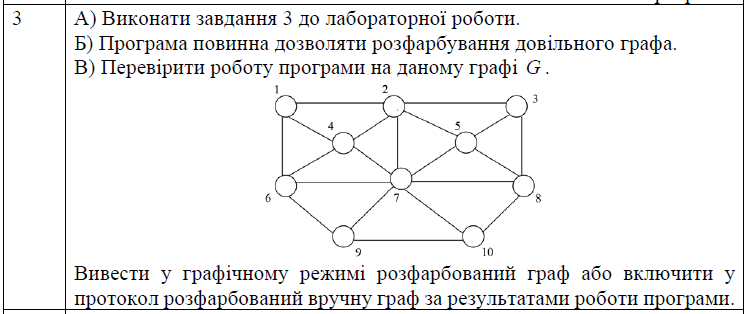
\includegraphics[width=0.7\textwidth]{photo1.png}
    \end{figure}

    \setlength{\parindent}{0pt}

    Блок-схема модифікованого евристичного алгоритму розфарбовування:

    \begin{figure}[ht]
        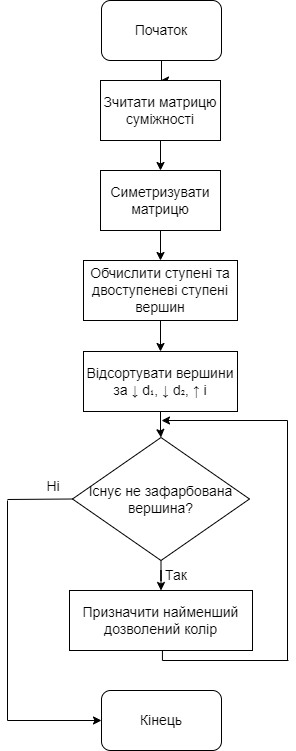
\includegraphics[width=0.326\textwidth]{diagram.png}
    \end{figure}

    \newpage

    \textbf{\underline{Код:}}

    \vspace{1em}

    {

    \begin{verbatim}
import tkinter as tk
from tkinter import filedialog, messagebox
import networkx as nx
import matplotlib.pyplot as plt
from matplotlib.backends.backend_tkagg import FigureCanvasTkAgg

CLASSIC_COLORS = [
    "red", "blue", "green", "yellow", "orange",
    "purple", "cyan", "magenta", "brown", "gray",
]

def read_matrix_from_file(filename: str) -> list[list[int]]:
    """Зчитати матрицю суміжності (цілі числа через пробіл) із файлу
*filename*."""
    with open(filename, "r", encoding="utf-8") as f:
        return [list(map(int, line.strip().split())) for line in f if
        line.strip()]

def to_undirected(matrix: list[list[int]]) -> list[list[int]]:
    """Повернути симетризовану (0/1) версію *matrix* для
неорієнтованого графа."""
    n = len(matrix)
    und = [[0] * n for _ in range(n)]
    for i in range(n):
        for j in range(n):
            if i != j and (matrix[i][j] or matrix[j][i]):
                und[i][j] = und[j][i] = 1
    return und


def modified_heuristic_coloring(matrix: list[list[int]]) -> list[int]:
    """Жадібне розфарбовування з упорядкуванням за ступенями (deg, 2‑step‑deg) на
неорієнтованому графі."""
    und = to_undirected(matrix)
    n = len(und)

    degree = [sum(row) for row in und]
    deg2 = [sum(degree[j] for j in range(n) if und[i][j]) for i in range(n)]

    order = sorted(range(n), key=lambda v: (-degree[v], -deg2[v], v))

    colour = [0] * n
    for v in order:
        forbidden = {colour[u] for u in range(n) if und[v][u] and colour[u]}
        c = 1
        while c in forbidden:
            c += 1
        colour[v] = c
    return colour

def draw_graph_colored(matrix: list[list[int]], colours: list[int]):
    """Намалювати граф із *matrix*, зафарбувавши вершини відповідно до *colours*
та палітри CLASSIC_COLORS."""
    und = to_undirected(matrix)
    n = len(und)
    G = nx.Graph()
    G.add_nodes_from(range(n))
    for i in range(n):
        for j in range(i + 1, n):
            if und[i][j]:
                G.add_edge(i, j)

    pos = nx.spring_layout(G)

    palette = [CLASSIC_COLORS[(c - 1) % len(CLASSIC_COLORS)] for c in colours]

    labels = {v: str(v + 1) for v in G.nodes()}

    nx.draw(
        G,
        pos,
        labels=labels,
        node_color=palette,
        node_size=600,
        font_color="white",
        edgecolors="black",
    )
    ax.set_title(f"Кількість кольорів: {max(colours)}")
    canvas.draw()

root = tk.Tk()
root.title("Модифікований евристичний алгоритм розфарбовування графа")

lbl_matrix = tk.Label(
    root,
    text="Матриця суміжності (наприклад: [[0,1,0],[1,0,1],[0,1,0]])",
)
lbl_matrix.pack(pady=(10, 0))

entry_matrix = tk.Text(root, height=6, width=60)
entry_matrix.pack()

for seq, virtual in {
    "<Control-c>": "<<Copy>>",
    "<Control-C>": "<<Copy>>",
    "<Control-v>": "<<Paste>>",
    "<Control-V>": "<<Paste>>",
    "<Control-x>": "<<Cut>>",
    "<Control-X>": "<<Cut>>",
}.items():
    entry_matrix.bind(seq, lambda e, v=virtual: entry_matrix.event_generate(v))

btn_load = tk.Button(root, text="Завантажити з файлу", command=lambda:
load_matrix_from_file())
btn_load.pack(pady=4)

btn_color = tk.Button(root, text="Розфарбувати граф", command=lambda:
run_coloring_from_input())
btn_color.pack()

label_result = tk.Label(root, text="", justify="left")
label_result.pack(pady=(6, 0))

fig, ax = plt.subplots(figsize=(5, 4))
canvas = FigureCanvasTkAgg(fig, master=root)
canvas.get_tk_widget().pack(pady=8)

def run_coloring_from_input():
    try:
        matrix = eval(entry_matrix.get("1.0", "end"))
        colours = modified_heuristic_coloring(matrix)

        ax.clear()
        draw_graph_colored(matrix, colours)

        result = "\n".join(
            f"Вершина {i + 1}: колір {colours[i]}" for i in range(len(colours))
        )
        label_result.config(text=result)
    except Exception as exc:
        messagebox.showerror("Помилка", str(exc))


def load_matrix_from_file():
    filename = filedialog.askopenfilename(
        title="Виберіть файл з матрицею", filetypes=[("Text files", "*.txt")]
    )
    if not filename:
        return
    try:
        matrix = read_matrix_from_file(filename)
        entry_matrix.delete("1.0", "end")
        entry_matrix.insert("1.0", str(matrix))
    except Exception as exc:
        messagebox.showerror("Помилка", str(exc))

root.mainloop()
    \end{verbatim}
}

    \newpage

    \textbf{\underline{Скріншот виконання програми:}}

    \begin{figure}[htbp]
        %--- верхній ряд ---
        \begin{subfigure}{0.35\textwidth}
            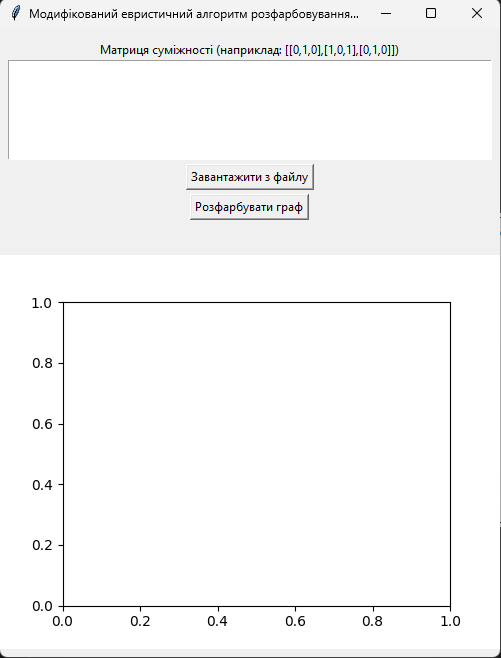
\includegraphics[width=\linewidth]{ex0.png}
            \label{fig:a}
        \end{subfigure}
        \begin{subfigure}{0.35\textwidth}
            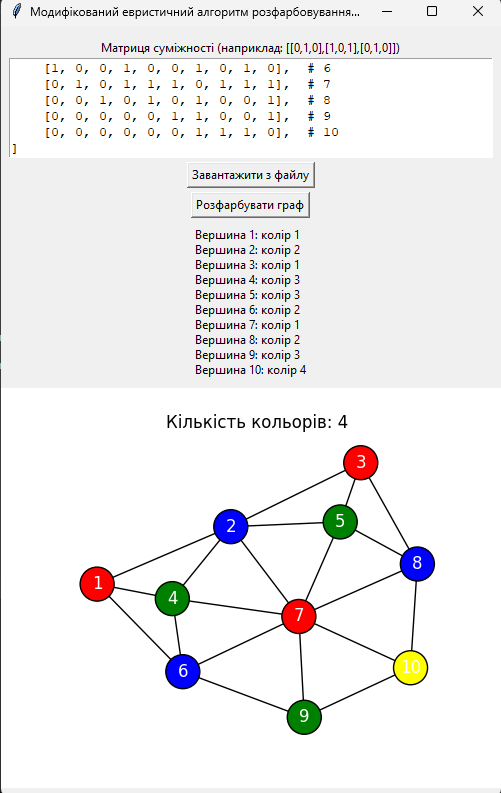
\includegraphics[width=\linewidth]{ex1.png}
            \label{fig:b}
        \end{subfigure}

        %--- нижній ряд ---
        \begin{subfigure}{0.35\textwidth}
            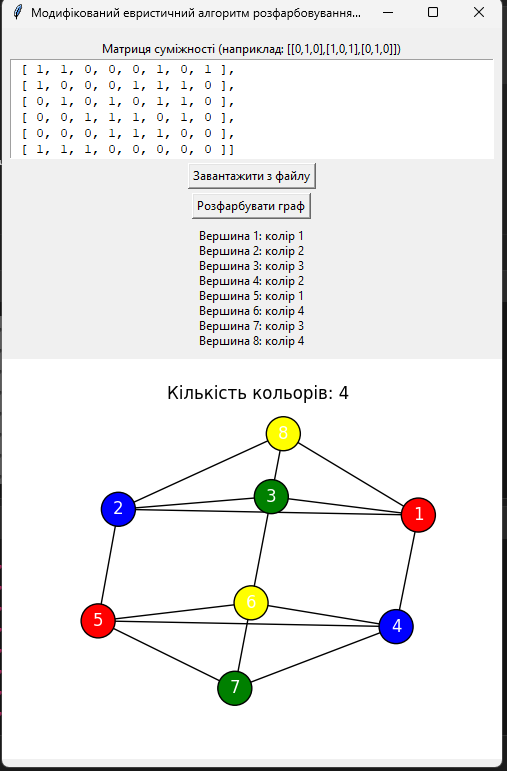
\includegraphics[width=\linewidth]{ex2.png}
            \label{fig:c}
        \end{subfigure}
        \begin{subfigure}{0.35\textwidth}
            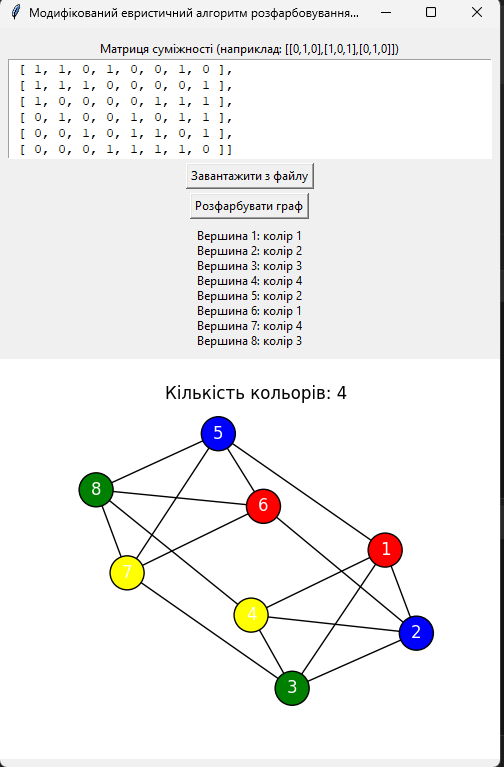
\includegraphics[width=\linewidth]{ex3.png}
            \label{fig:d}
        \end{subfigure}

        \label{fig:grid4}
    \end{figure}

    \textbf{\underline{Висновок:}}
    У ході виконання лабораторної роботи №4 було розглянуто задачу розфарбовування графа та реалізовано модифікований жадібний алгоритм розфарбовування. Були вивчені основні теоретичні поняття: граф, матриця суміжності, ступінь вершини, хроматичне число та двоступеневий ступінь.
    Розроблений алгоритм дозволяє ефективно розфарбовувати неорієнтовані графи, враховуючи як локальні характеристики вершини (її ступінь), так і структуру її оточення (двоступеневий ступінь). Це дає змогу покращити порядок розфарбування та зменшити кількість використаних кольорів у порівнянні з класичним жадібним підходом.
    Практична реалізація на Python із використанням бібліотек \texttt{networkx}, \texttt{matplotlib} і \texttt{tkinter} дозволила наочно перевірити роботу алгоритму на графах довільної структури.

\end{document}